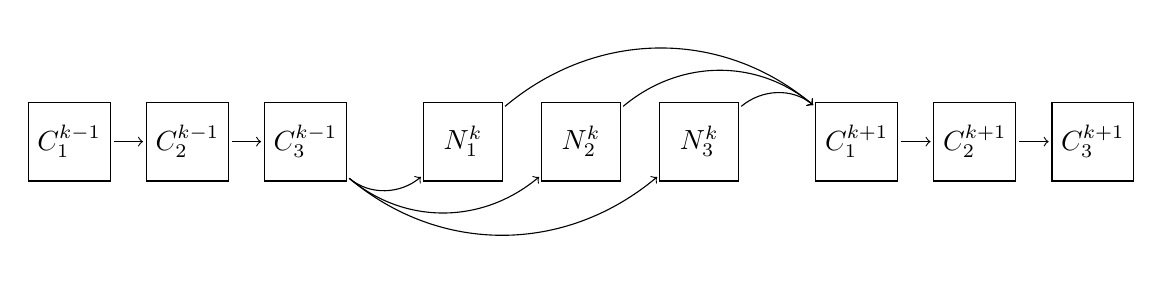
\begin{tikzpicture}
    \node[style=draw, minimum width=1cm, minimum height=1cm] (c1) at (0, 0) {$C^{k-1}_1$};
    \node[style=draw, minimum width=1cm, minimum height=1cm] (c2) at (1.5, 0) {$C^{k-1}_2$};
    \node[style=draw, minimum width=1cm, minimum height=1cm] (c3) at (3, 0) {$C^{k-1}_3$};

    \node[style=draw, minimum width=1cm, minimum height=1cm] (n1) at (5, 0) {$N^k_1$};
    \node[style=draw, minimum width=1cm, minimum height=1cm] (n2) at (6.5, 0) {$N^k_2$};
    \node[style=draw, minimum width=1cm, minimum height=1cm] (n3) at (8, 0) {$N^k_3$};

    \node[style=draw, minimum width=1cm, minimum height=1cm] (c4) at (10, 0) {$C^{k+1}_1$};
    \node[style=draw, minimum width=1cm, minimum height=1cm] (c5) at (11.5, 0) {$C^{k+1}_2$};
    \node[style=draw, minimum width=1cm, minimum height=1cm] (c6) at (13, 0) {$C^{k+1}_3$};

    \draw[->, shorten >=1pt, shorten <=1pt] (c1) -- (c2);
    \draw[->, shorten >=1pt, shorten <=1pt] (c2) -- (c3);

    \draw[->, shorten >=1pt, shorten <=1pt] (c3) to[out=320,in=220] (n1);
    \draw[->, shorten >=1pt, shorten <=1pt] (c3) to[out=320,in=220] (n2);
    \draw[->, shorten >=1pt, shorten <=1pt] (c3) to[out=320,in=220] (n3);

    \draw[->, shorten >=1pt, shorten <=1pt] (n1) to[out=40,in=140] (c4);
    \draw[->, shorten >=1pt, shorten <=1pt] (n2) to[out=40,in=140] (c4);
    \draw[->, shorten >=1pt, shorten <=1pt] (n3) to[out=40,in=140] (c4);

    \draw[->, shorten >=1pt, shorten <=1pt] (c4) -- (c5);
    \draw[->, shorten >=1pt, shorten <=1pt] (c5) -- (c6);
\end{tikzpicture}